\chapter{Speaker counting}
\label{chap:counting}

\lettrine{I}{n} this chapter, we present our speaker counting system and the experiments that we carry out to demonstrate and improve its robustness. Inspired by a pioneering work on speaker counting with neural networks \cite{stoter_countnet:_2019}, we design a CRNN that is capable of counting up to 5 speakers in a multi-channel mixture containing noise and reverberation. We describe the input representation adopted to feed the neural network and how we address speaker counting as a classification problem. We detail the generation of the dataset used for training the network, as well as the testing datasets, the baseline systems and the metrics employed for assessing speaker counting performance. Finally, we present the different experiments we conduct with this system, and report and comment the results. The first series of experiments focus on assessing the use of multi-channel over single-channel signals, the second one compares the use of different convolution kernel sizes, and the last one is a short analysis which examines the network prediction accuracy depending on the considered frame in a given input sequence.

%-----------------------------------------------
%  OVERALL METHODOLOGY
%-----------------------------------------------
\section{Overall methodology}

\subsection{Input features}

As one can intuit, spectral information is important to distinguish between several overlapping speakers, and thus, for counting how many they are. This is why in \cite{stoter_countnet:_2019} the authors chose to represent the single-channel input signal with a time-frequency representation, in the STFT domain, leading to the use of the magnitude spectrogram. In our case, we want to add spatial information to our representation, which we conjecture to be useful for the network to better distinguish multiple speakers. This is why we represent the input signal with the multi-channel Ambisonics format, limited to order 1 (FOA). Recalling \eqref{eq:foaSTFT}, an FOA signal in the STFT domain is encoded with four (complex-valued) STFT representations, from which we extract the magnitude information to obtain a 4-channel magnitude spectrogram. As it was done in \cite{stoter_countnet:_2019}, we discard the phase information, which is also justified by the use of the Ambisonics format, which is theoretically obtained with coincident microphones.

Since a magnitude spectrogram is a TF representation, it is generally represented in the form of 2D matrices of size $T \times F$, where $T$ is the number of frames and $F$ the number of frequency bins up to the Nyquist frequency. In our representation, the four channels of the FOA magnitude spectrogram are stacked together in a third dimension leading to a 3D input tensor $\mathbf{X} \in \mathbb{R}^{T \times F \times 4}$. Fig.~\ref{fig:foaMagnitudeSpectrograms} shows an example of the 4-channel magnitude spectrogram obtained for an input signal.

\begin{figure}[t]
    \begin{center}
    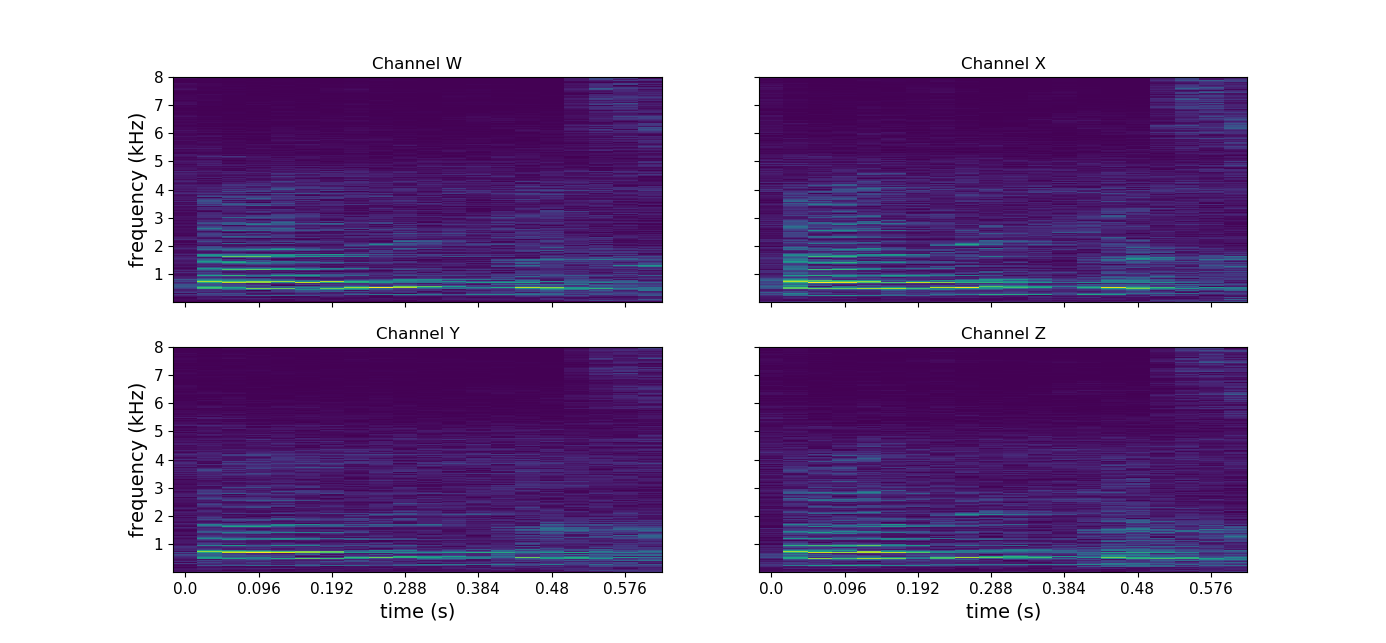
\includegraphics[width=1.\linewidth]{Images/chap5/foaMagnitudeSpectrograms.png}
    \captionof{figure}[Example of an input signal represented with a FOA magnitude spectrogram]{Example of an input signal represented with a FOA magnitude spectrogram. In this example, $T = 20$, and the number of speakers (which is difficult to estimate visually) is $1$ from $0$ to $0.372$~s and $2$ for the remaining frames. For a better visualization, we apply a log function to these spectrograms, but in practice it is not done during the experiments.}
    \label{fig:foaMagnitudeSpectrograms}
    \end{center}
\end{figure}

As it is usual in deep learning, we normalize these spectrograms per frequency band over the entire training dataset, so that the mean and variance for each frequency band (including all frames and channels) are $0$ and $1$, respectively. The same mean and variance values from the training dataset are used to normalize the test data.

\subsection{Speaker counting as a classification problem}

We consider speaker counting as a multi-class classification problem, as it was shown to be more efficient than regression \cite{stoter_classification_2018}. Each class represents a number of speakers, and the network is trained to evaluate the probability of the input feature to belong to that class. More specifically, we limit our speaker counting system to count between $0$ and $5$ speakers, leading to $6$ potential classes $c_i$, $i \in \{0,1,2,3,4,5\}$. Then, for each input frame, the neural network is trained to estimate the probability $P(t,c_i \mid \mathbf{X})$ that the $t$-frame belongs to class $c_i$, and for $i \in \{0,1,2,3,4,5\}$ (\emph{i.e.}, it output $6$ values in $[0,1]$), as illustrated in Fig.~\ref{fig:countingClassification}. As detailed further, we design the network output layer so that all outputs sum to $1$, acting as a discrete probability distribution. Finally, the number of speakers for the considered frame is estimated by selecting the class with the highest probability:
\begin{equation}
    \hat{J}(t) = \argmax_i P(t,c_i \mid \mathbf{X}).
\end{equation}
 
\begin{figure}[t]
    \begin{center}
    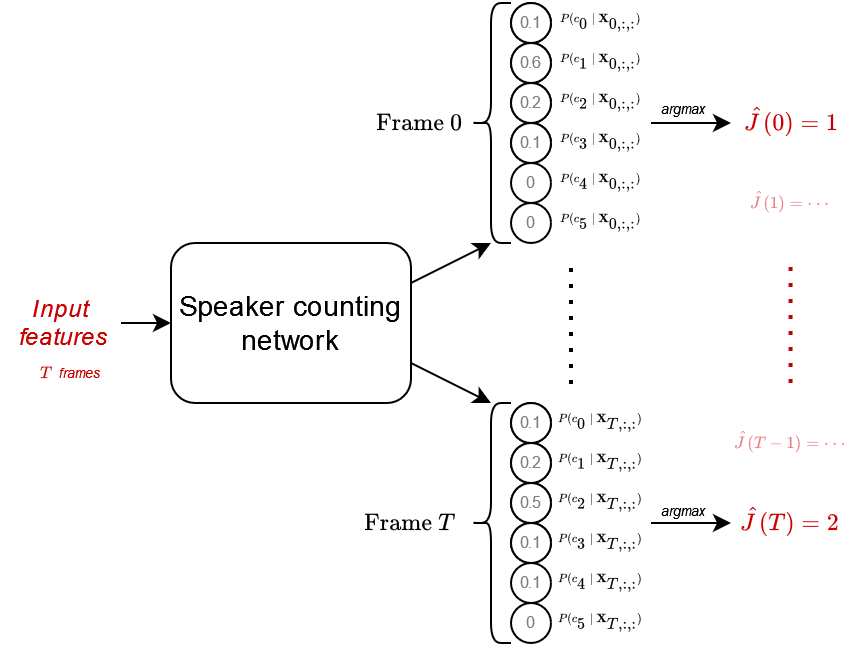
\includegraphics[width=0.9\linewidth]{Images/chap5/countingClassification.png}
    \captionof{figure}[Speaker counting as a classification problem]{Speaker counting as a classification problem. Each candidate number of speakers is considered as a class, and the neural network is trained to estimate the probability that the input feature belongs to each class. The neural network is forced to output the set of probabilities for each frame in the input feature.}
    \label{fig:countingClassification}
    \end{center}
\end{figure}

Note that in our method, a probability for each class is computed for each frame, leading to a frame-wise resolution for our counting system. This is the main difference with \cite{stoter_classification_2018}, in which the authors proposed to calculate a single probability distribution for the whole $5$-s long input sequence.

\subsection{Neural network global architecture}
\label{ss:countingNetworkArchitecture}

The neural network architecture we adopt for speaker counting is inspired by \cite{stoter_countnet:_2019}, and is illustrated on Fig.~\ref{fig:countingNetworkArchitecture}.

A first series of convolutional layers processes the input tensor of shape $T \times 513 \times 4$ (the value $513$, which is the number of frequency bins, comes from the chosen STFT analysis window size, see Section~\ref{ss:countingAudioParameters}), where $T$ is an hyperparameter in our experiments, and performs a feature extraction. This convolutional block first consists of two 2D convolutional layers with 64 and 32 convolution kernels of size $K \times K$, respectively, applied on the temporal and frequency axes, where $K$ is another hyperparameter in our experiments. Then, a max-pooling layer with a pooling size of $1 \times 3$ is used, in order to preserve the information along the temporal axis. Next, two other 2D convolutional layers with respectively 128 and 64 convolution kernels of size $K \times K$ are used, followed by another max-pooling layer of size $1 \times 3$. In all convolutional layers, we use a stride of 1 as well as zero-padding in order to preserve the shape of the input tensor. The important change compared to \cite{stoter_countnet:_2019} is that we use a max-pooling $1 \times 3$ instead of $3 \times 3$, allowing us to preserve the temporal dimension for a prediction at a frame-wise resolution.

The new features extracted by the convolutional module consist of $64$ feature maps of size $T \times 57$. In order to proceed to a temporal analysis with recurrent layers, we reshape the obtained feature by stacking the feature maps along its second dimension, leading to a reshaped feature of size $T \times 3648$. In all convolutional layers, ReLU activations are used. Batch normalization is also applied before each max-pooling layer to make the neural network faster and more stable.

The temporal processing is then done using a single LSTM layer with a hidden state vector size of $40$. This LSTM layer is used in a sequence-to-sequence mode, \emph{i.e.}, the hidden state of the LSTM cell is output at each timestep, so that we obtain a new vector for each item of the input sequence (which is of length $T$). The activation functions used in the LSTM cells are the same as described in Section~\ref{ss:lstm}, \emph{i.e.}, $\sigma_h$ is the hyperbolic tangent function and $\sigma_s$ is the sigmoid function.

Finally, each vector from the output sequence of the LSTM layer is processed independently by the 6-neuron output feedforward layer, whose activation is set to the softmax function. This ensures that a probability distribution over the $6$ classes is produced for each timestep.

\begin{figure}[t]
    \begin{center}
    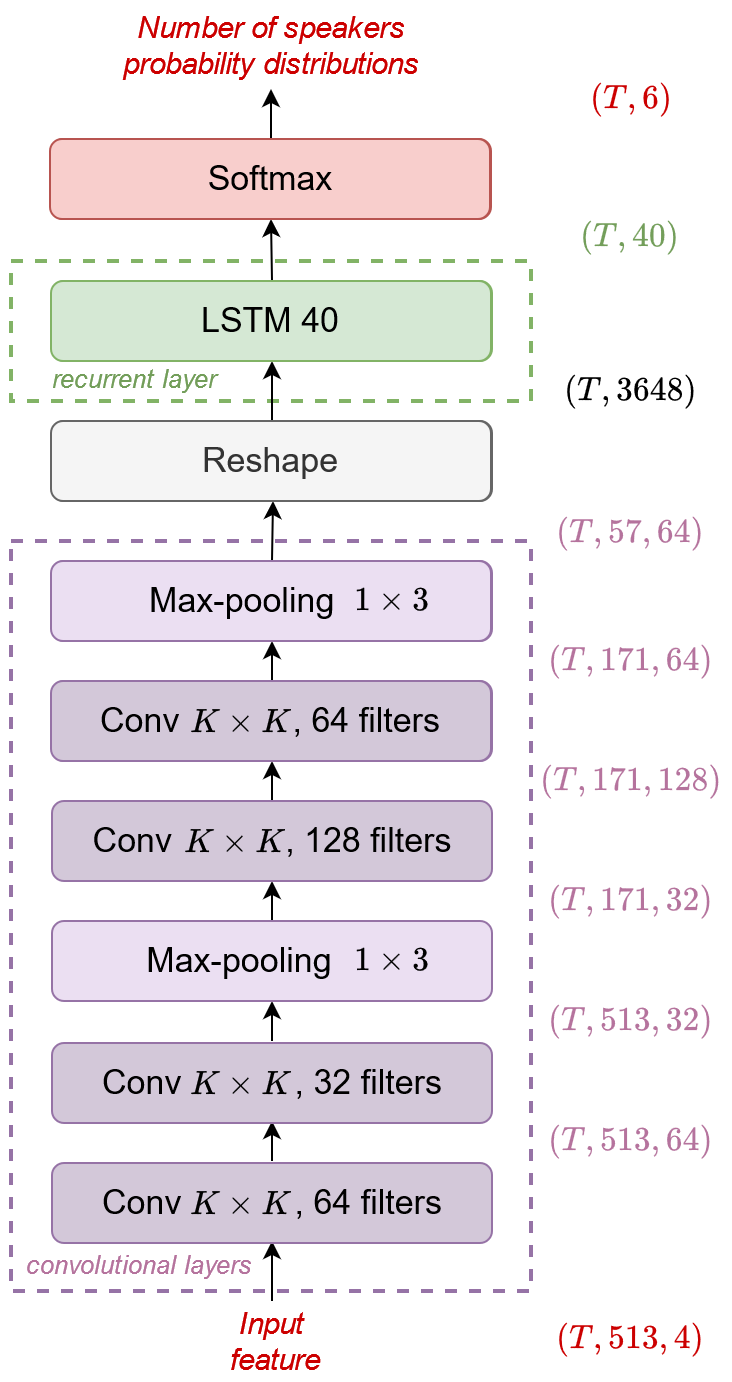
\includegraphics[width=0.4\linewidth]{Images/chap5/countingNetworkArchitecture.png}
    \captionof{figure}[Neural network architecture for speaker counting]{Neural network architecture for speaker counting. It is composed of a series of 2D convolutional layers, with max-pooling layers in-between, followed by an LSTM layer and a feedforward layer acting as the output layer. Max-pooling is applied only on the second axis (corresponding to the frequency dimension) to preserve temporal dimensionality and the LSTM is used in a sequence-to-sequence mode. The convolution kernel size $K \times K$ and the number of frames $T$ in the input features are hyperparameters in our experiments.}
    \label{fig:countingNetworkArchitecture}
    \end{center}
\end{figure}

%-----------------------------------------------
%  EXPERIMENTAL PROTOCOL
%-----------------------------------------------
\section{Experimental protocol}
\subsection{Audio parameters}
\label{ss:countingAudioParameters}

In our experiments, the audio signals are sampled at $16$~kHz, which is the frequency range of the Eigenmike\textsuperscript{\textregistered} array for which the FOA channels exhibit acceptable directivity distortion \cite{baque_analyse_2017}. The STFT is computed using a sinusoidal window of length $1\,024$ ($64$~ms) with an overlap of $50$\%, thus a frame is computed every $32$~ms. The FFT size is also $1\,024$, leading to $513$ frequency bins. 

\subsection{Training parameters}

The loss function used for training is the categorical cross-entropy. The Adam optimizer \cite{kingma_adam:_2014} is used with a starting learning rate of $10^{-3}$, $\beta_1 = 0.9$, $\beta_2=0.999$, $\epsilon = 10^{-7}$. During the training phase, a dropout is used before the reshape layer, with a dropout rate of $0.25$. During training, we monitor the categorical accuracy on the validation set, and we stop the training if the accuracy has not improved for $20$ epochs, keeping the model with the best accuracy so far. The maximum number of epochs is set to $300$. When the validation accuracy has not improved for 10 epochs, we divide the learning rate by a factor $2$.

\subsection{Training data}
\label{ss:countingTrainingData}

Our speaker counting CRNN is trained on simulated data. The simulation can be decomposed into two phases: the generation of RIRs and the generation of the training signals.

The RIRs are simulated with the image-source method \cite{allen_image_1979}, by adapting an existing framework \cite{habets_room_2006} to generate FOA RIRs. A large number of RIRs are generated in a variety of random conditions, such as the room dimensions and absorption coefficients, the microphone and source positions. First, we randomly set the dimension of the room, which is simplified to be parallelepipedic (usually referred to as a \textit{shoebox}), within $[2,10]$~m, $[2,10]$~m and $[2,3]$~m, for the length, width and height, respectively. The room RT60 is randomly chosen between $200$ and $800$~ms. Next, an ideal (open sphere) spherical microphone is randomly positioned in the room so that it is at least at a distance of $0.5$~m from the walls. Then, $5$ source positions are randomly picked within the room dimensions. The protocol is repeated for $10\,000$ rooms, so that we end up with $50\,000$ RIRs.

To generate the speech mixtures, we use $16$-kHz speech excerpts from the TIMIT dataset \cite{garofolo_timit_1993}. To match realistic conditions, we want to generate conversation-like mixtures, with the instantaneous number of speakers (in between $0$ and $5$) varying over time. The speech mixtures also need to be generated as if the speakers were in the same room (hence the $5$ generated RIRs per room). To create such a realistic signal, we first fix a total number of speakers $J$ which will participate in the current speech mixture (between $1$ and $5$). To create the mixture, a single-speaker $15$~s dry signal is first generated by concatenating several sentences from a unique random speaker in the TIMIT database (it is crucial in this step not to mix sentences from different speakers to ensure the continuity of one speaker's frequency content) and alternating actual speech content with silence segments. More specifically, a preliminary silence with a random length in $[0.5,1]$~s first initializes the signal. Then a random sentence from the chosen speaker is concatenated with the signal, followed by a silence of random length in $[0.5,2]$~s. This last step is repeated for random sentences until a $15$~s signal is obtained.\footnote{If the last concatenated sentence is too long so that the signal will be longer than $15$~s, it is cropped and faded out in the last $100$~ms.} The obtained single-speaker $15$~s dry signal is then convolved with one RIR of a randomly picked room to create a wet signal. This process is repeated for the $J$ speakers of the current mixture, using the $J$ distinct RIRs from the same room. Then, we mix all the single-speaker wet signals together to create a speech mixture with an instantaneous number of speakers varying from $0$ to $J$ speakers. The signal-to-interference ratios (SIR) used between the first single-speaker signal and the other signals is randomly chosen in $[0,10]$~dB. The last step is to add a diffuse noise to this mixture to make it a step further more realistic. We randomly choose a noise signal among those in a noise database constituted from various signals from Freesound\footnote{https://freesound.org/} (including crowd, traffic, engine, nature sounds, etc.), which we convolve with a diffuse field generated by averaging the diffuse parts of two random RIRs measured in a real reverberant room. A random SNR is picked in $[0,20]$~dB with respect to the first speech signal.

In the TIMIT dataset, each speech sentence is annotated with the pronounced word timestamps, at a sample precision. We use these annotations to automatically label voice activity vs silence for each speaker and thus label the $15$~s mixtures with the ground-truth number of speakers at the sample resolution. When these signals are transformed into the STFT domain, we consider that a speaker is active in a frame if it is active for more than half of the samples in that frame.

Fig.~\ref{fig:spectrogramsWithVaryingNOS} illustrates three examples of a $15$~s mixture with a varying number of speakers. Because each speaker randomly starts and stops uttering small sentences, the number of speakers varies several times along the sequence.

\begin{figure}[t]
    \begin{center}
    \makebox[\textwidth][c]{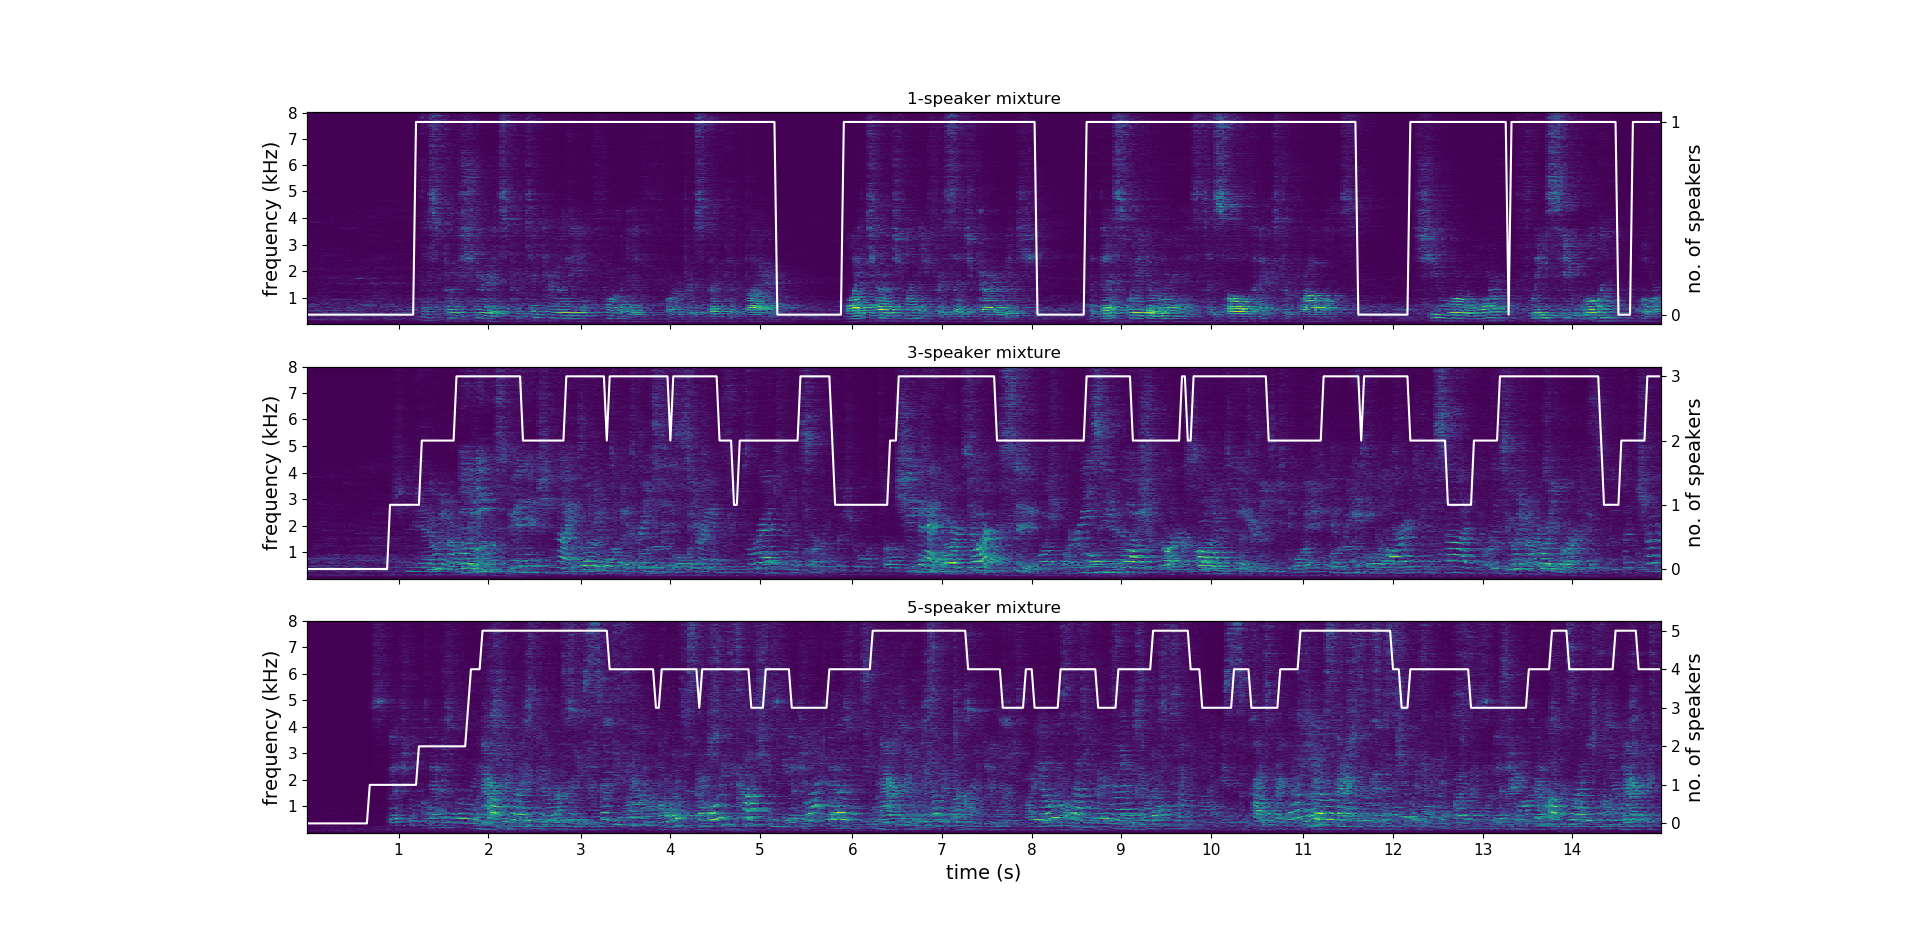
\includegraphics[width=1.4\linewidth]{Images/chap5/spectrogramsWithVaryingNOS.png}}
    \captionof{figure}[Example of spectrograms of $15$~s long signals with varying number of speakers]{Example of spectrograms ($W$ channel only) of $15$~s long training signals with varying number of speakers. The white lines represent the varying (ground-truth) number of speakers in each mixture. The maximum number of speakers in these mixture are $1$ (top), $3$ (middle) and $5$ (bottom). As we can see, the instantaneous number of speakers ``continuously'' varies along the $15$~s of mixture, as each speaker starts and stops uttering a small sentence all along the signal.}
    \label{fig:spectrogramsWithVaryingNOS}
    \end{center}
\end{figure}

We recall that each (train or test) input feature to our network is a sequence of $T$ consecutive 4-channel FOA STFT magnitude frames, with $T$ an hyperparameter that we set experimentally. These sequences are extracted from these $15$~s mixtures with basic segmentation, without any overlap between the sequences.
The first version of our training dataset consisted of 5 $J$-speaker $15$-s mixtures, for $J \in \{1,2,3,4,5\}$, for each room, leading to the same number of training/test sequences for each number of speaker $J$. However this strategy actually raises the famous \textit{class imbalance problem} \cite{buda_systematic_2018}, which happens when the number of examples is very different for each class. As we can see in the plots on Fig.~\ref{fig:spectrogramsWithVaryingNOS}, in each mixture the instantaneous number of speakers fluctuates around certain values and rarely reaches others. For example, in the $3$-speaker mixture, the number of speakers is most often $2$ or $3$, while in the bottom plot we see that there barely are $5$-speaker frames. Globally, generating the exact same number of $J$-speaker mixtures for all values of $J$ would unbalance the cardinality of each class, with more training data towards the low-valued classes. To avoid this problem, we decide not to systematically generate all $5$ speech mixtures for each room, but rather setting a probability that a $J$-speaker mixture will actually be generated. Table~\ref{tab:NOSgenerationProbabilities} shows these probabilities, set empirically to attain a more balanced training dataset. To illustrate this process, let us assume we already selected a certain room configuration, which comes with $5$ generated SRIRs. We first consider a $1$-speaker mixture, which probability of generation is $0.2$ as indicated in Table~\ref{tab:NOSgenerationProbabilities}. Whether the draw leads to the actual mixture generation or not, we then consider the generation of a $2$-speaker mixture, this time with a probability of $0.3$. We continue in this process until considering the generation of a $5$-speaker mixture, which is actually always done because of the probability $1$. In that manner, we have actually generated $1$-speaker mixtures using $1$ SRIR from only $20$\% of the considered rooms, $2$-speaker mixtures using $2$ SRIRs from only $30$\% of the rooms, etc.


\begin{table}[t]
\centering
\begin{tabular}{|c|ccccc|}
\hline
\textbf{$J$}                                                                                                      & \textbf{1}           & \textbf{2}           & \textbf{3}           & \textbf{4}           & \textbf{5}         \\ \hline
\multirow{2}{*}{\textbf{\begin{tabular}[c]{@{}c@{}}Probability to generate\\ a $J$-speaker mixture\end{tabular}}} & \multirow{2}{*}{0.2} & \multirow{2}{*}{0.3} & \multirow{2}{*}{0.4} & \multirow{2}{*}{0.5} & \multirow{2}{*}{1} \\
                                                                                                                  &                      &                      &                      &                      &                    \\ \hline
\end{tabular}
\captionof{table}[Probabilities of generating a $J$-speaker mixture]{Probabilities of generating a $J$-speaker mixture during the creation of the training dataset.}
\label{tab:NOSgenerationProbabilities}
\end{table}

The validation dataset, used to monitor the neural network training, is created exactly with the same methodology. Only $100$ rooms are considered for this dataset, and we took care not to use generation data already used for the training dataset (speech sentences, speaker identities, rooms, noise signals).

Finally, we end up with about $100$~hours of training data and $1$~hour of validation data.

\subsection{Testing data}
\label{ss:countingTestingData}

The test dataset used to assess our models is a simulated dataset created in the same manner as the training and validation datasets. For the test, we generated $500$ RIRs in $100$ different rooms. Again, the speakers and noise signals used for the test signals have not been used for the training and validation datasets. The obtained test dataset contains $1$~hour of data. 

\subsection{Baseline}

As our speaker counting system is partly inspired by the classification-based CRNN proposed in \cite{stoter_countnet:_2019}, we consider this method as a baseline for the experiment in which we compare the use of single- and multi-channel signals. We nevertheless adjust this baseline to ensure having a fair comparison to our method. First, we employ the recurrent layer in a sequence-to-sequence manner so that a prediction is made for every frame in the input feature.\footnote{In \cite{stoter_countnet:_2019}, the authors designed their network to produce only one prediction for the whole input feature, as their goal was to predict the maximum number of speakers present in a $5$-s single-channel mixture.} This choice constraints us to use max-pooling of size $1 \times 3$ instead of $3 \times 3$ to preserve the temporal dimension.


\subsection{Evaluation metrics}

To measure the performance of our speaker counting system we use several metrics. The classification accuracy $A_{ii}$ for one class $c_i$ is defined by the percentage of frames correctly classified with class $c_i$, among all frames belonging to class $c_i$. While it is a usual metric in a classification problem, we also extend this metric to measure the percentage of frames that are classified with class $c_j$ among all frames belonging to class $c_i$. Hereafter, $A$ is referred as the confusion matrix. Mathematically, by noting $T_i$ the set of all test frames indices with the ground-truth number of speakers equal to $i$, $A_{ij}$ is expressed as:
\begin{equation}
    A_{ij} = \frac{\mathsf{card}(\{t \in T_i \mid \hat{J}(t) = j\})}{\mathsf{card}(T_i)},
\end{equation}
where $\mathsf{card}(T_i)$ denotes the cardinality of the set $T_i$.
This accuracy metric calculated according to two indices (each representing a NoS) will be useful to assess how far the estimated number of speakers deviates from the ground-truth value. 

We also measure the mean absolute error $M_i$ per class, which is defined as:
\begin{equation}
    M_i = \frac{1}{\mathsf{card}(T_i)} \sum_{t \in T_i} \lvert \hat{J}(t) - J(t) \rvert.
\end{equation}

%-----------------------------------------------
%  EXPERIMENTS
%-----------------------------------------------
\section{Experiments}

In this section, we report and discuss the results of our speaker counting CRNN evaluation. We conduct several experiments in which we assess the values of some hyperparameters: the benefit of using multi-channel signals, the number of frames in the input sequence, the convolution kernel sizes. We also propose an analysis of the accuracy of the network depending on the frame position within the input sequence.

\subsection{Single-channel against multi-channel features, with several sequence lengths}

\subsubsection{Experiment objective}

The preliminary objective of our speaking counting CRNN is to assess the benefit of using multi-channel signals over single-channel ones, such as the one proposed in \cite{stoter_countnet:_2019}. As explained above, we adapt this baseline network to our problem of estimating the instantaneous number of speakers. Therefore, the baseline in this experiment is the same speaker counting architecture we adopt, presented in Section~\ref{ss:countingNetworkArchitecture}, but we limit the input features to only one channel. Instead of using the $4$ channels obtained from the FOA representation, only the $W$ channel is considered for the baseline. The $W$ channel encodes the recorded signal as if it was recorded by an omnidirectional microphone, which can be adequately considered as a single-channel representation. 

\begin{figure}[t]
    \centering
    \makebox[\textwidth][c]{
    \subfloat[Single-channel,\\ 10 frames]{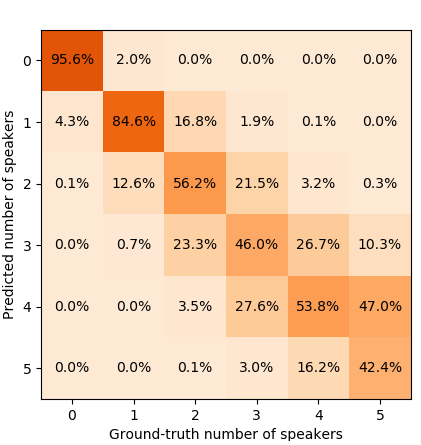
\includegraphics[width=.4\textwidth]{Images/chap5/conf_mat_mono_10frames_simulatedSRIRs.png} \label{subfig:cm_mono_10frames_sim}}
    \subfloat[Single-channel,\\ 20 frames]{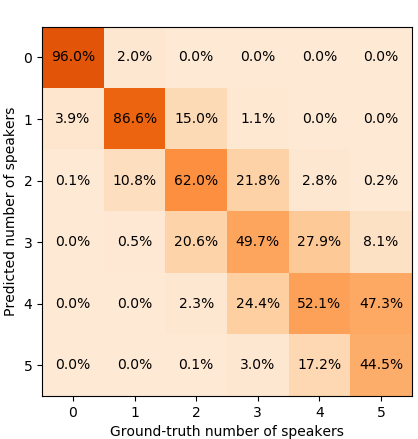
\includegraphics[width=.4\textwidth]{Images/chap5/conf_mat_mono_20frames_simulatedSRIRs.png} \label{subfig:cm_mono_20frames_sim}}
    \subfloat[Single-channel,\\ 30 frames]{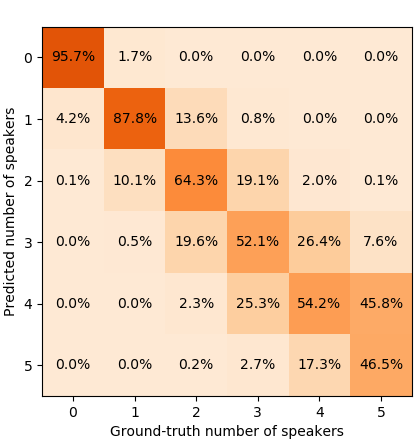
\includegraphics[width=.4\textwidth]{Images/chap5/conf_mat_mono_30frames_simulatedSRIRs.png} \label{subfig:cm_mono_30frames_sim}}}\\
    
    \makebox[\textwidth][c]{
    \subfloat[Multi-channel,\\ 10 frames]{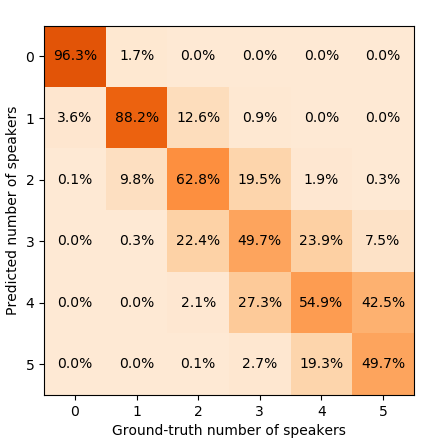
\includegraphics[width=.4\textwidth]{Images/chap5/conf_mat_multi_10frames_simulatedSRIRs.png} \label{subfig:cm_multi_10frames_sim}}
    \subfloat[Multi-channel,\\ 20 frames]{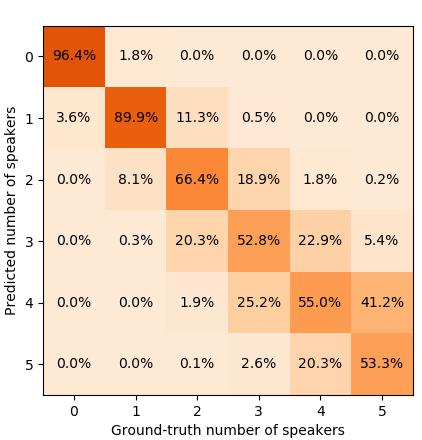
\includegraphics[width=.4\textwidth]{Images/chap5/conf_mat_multi_20frames_simulatedSRIRs.png} \label{subfig:cm_multi_20frames_sim}}
    \subfloat[Multi-channel,\\ 30 frames]{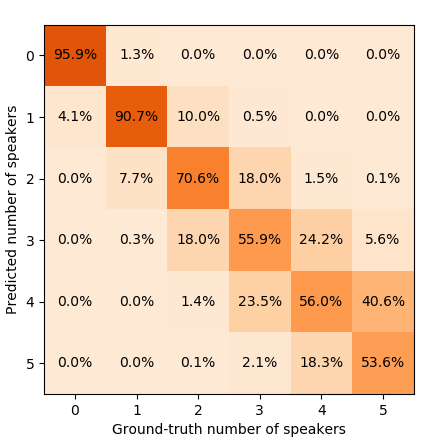
\includegraphics[width=.4\textwidth]{Images/chap5/conf_mat_multi_30frames_simulatedSRIRs.png} \label{subfig:cm_multi_30frames_sim}}}
    
    \captionof{figure}[Confusion matrix $A_{ij}$ of the single-channel and multi-channel speaker counting CRNNs on the test dataset with simulated SRIRs, for several values of $T$]{Confusion matrix $A_{ij}$ of the single-channel (top) and multi-channel (bottom) speaker counting CRNNs on the test dataset with simulated SRIRs, for $T = 10, 20, 30$~frames (left to right).}
    \label{fig:confusionMatricesSingleMultiSimulated}
\end{figure}

The intuition behind using multi-channel features is to provide the neural network with a means to better discriminate between spatially distinct sources. As it is done in source localization (see Chapter~\ref{chap:multisourceLocalization}), feeding multi-channel features to the neural network supplies it with multiple transformed versions of the same signal (due to the different microphone types and orientations). Depending on the source location, the original signal is not transformed the same way, which should be reflected in the magnitude spectrogram. We conjecture that the neural network can learn these characteristics to better discriminate the different speech sources.

To compare the use of single- and multi-channel features in several conditions, we also vary the length of the input sequence, \emph{i.e.}, the number of frames $T$ in the input features. We experimented with $T=10$ ($320$~ms), $T=20$ ($640$~ms), and $T=30$ ($\approx 1$~s). In this experiment, the convolution kernel size is $K=3$ (see Section~\ref{ss:countingConvolutionExperiment} for an experiment on this hyperparameter).

\subsubsection{Results}

\begin{figure}[t]
    \centering
    \makebox[\textwidth][c]{
    \subfloat[Single-channel,\\ 10 frames]{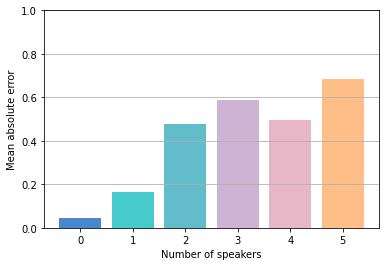
\includegraphics[width=.4\textwidth]{Images/chap5/mae_mono_10frames_simulatedSRIRs.png} \label{subfig:mae_mono_10frames_sim}}
    \subfloat[Single-channel,\\ 20 frames]{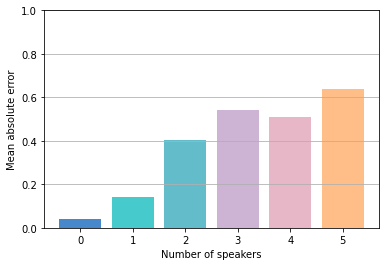
\includegraphics[width=.4\textwidth]{Images/chap5/mae_mono_20frames_simulatedSRIRs.png} \label{subfig:mae_mono_20frames_sim}}
    \subfloat[Single-channel,\\ 30 frames]{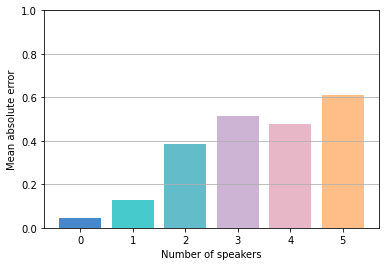
\includegraphics[width=.4\textwidth]{Images/chap5/mae_mono_30frames_simulatedSRIRs.png} \label{subfig:mae_mono_30frames_sim}}}\\
    
    \makebox[\textwidth][c]{
    \subfloat[Multi-channel,\\ 10 frames]{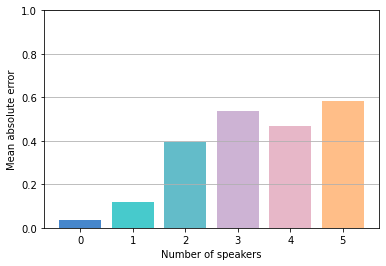
\includegraphics[width=.4\textwidth]{Images/chap5/mae_multi_10frames_simulatedSRIRs.png} \label{subfig:mae_multi_10frames_sim}}
    \subfloat[Multi-channel,\\ 20 frames]{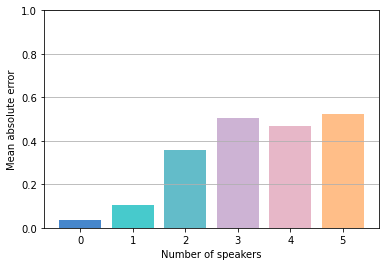
\includegraphics[width=.4\textwidth]{Images/chap5/mae_multi_20frames_simulatedSRIRs.png} \label{subfig:mae_multi_20frames_sim}}
    \subfloat[Multi-channel,\\ 30 frames]{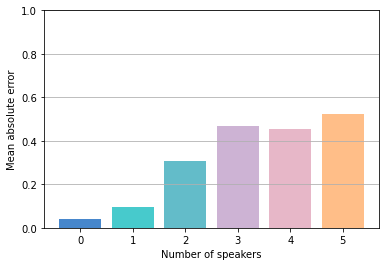
\includegraphics[width=.4\textwidth]{Images/chap5/mae_multi_30frames_simulatedSRIRs.png} \label{subfig:mae_multi_30frames_sim}}}
    
    \captionof{figure}[Mean absolute errors $M_i$ of the single-channel and multi-channel speaker counting CRNNs on the test dataset with simulated SRIRs, for several values of $T$]{Mean absolute errors $M_i$ of the single-channel and multi-channel speaker counting CRNNs on the test dataset with simulated SRIRs, for $T = 10, 20, 30$~frames (left to right).}
    \label{fig:maeSingleMultiSimulated}
\end{figure}


We report the detailed accuracy results for all $6$ experiments in the form of confusion matrices, which display the percentage of $j$-speaker frames (on the x-axis) which are estimated to contain $j$ speakers (on the y-axis). These confusion matrices are shown in Figure~\ref{fig:confusionMatricesSingleMultiSimulated}. We also report graphics of the mean absolute errors in Figure~\ref{fig:maeSingleMultiSimulated}. We recall that we compare the use of single-channel features to multi-channel features, for $3$ values of $T$: $10$, $20$ and $30$ frames.

First, we notice that both single- and multi-channel networks are very effective to detect the absence of speech in the signal, with over $95$\% of correct silent detection in all settings. It can therefore act as a robust VAD system. Then, the classification accuracy gradually decreases when the number of speakers increases, which is anticipated since the task becomes more complex. While the classification accuracy for $1$-speaker signals is around $85$\% for the single-channel network, it reaches around $44$\% accuracy when $5$ speakers are present in the signal, which is still an acceptable performance compared to a random guessing accuracy ($16$\%). 

While the mean absolute error is almost zero for zero-speaker signals in all configurations, it remains under $0.8$ when one or more speakers are active, which means that when the neural network predicts a wrong number of speakers, the error is $\pm 1$ speaker in average. This behavior can be clearly noticed in the confusion matrices. When the network's prediction is wrong it is almost always done with an absolute error of $1$, which is visualized around the matrix diagonal. For example, in Fig.~\ref{subfig:cm_multi_20frames_sim}, we see that when the ground-truth number of speakers is $3$, the neural network predicts wrongly $2$ speakers $18.9$\% of the time and $4$ speakers $25.2$\%, while it estimates $0$, $1$ or $5$ only $3.1$\% of the time in total. Regarding the class $J=5$ speakers, there seems to be an \textit{edge effect}, so that the number of prediction for $J-1$ speakers is surprisingly high compared to the other values of $J$, but this can be explained because of the absence of the class $J=6$.

When comparing the effectiveness of the single- and multi-channel settings, we clearly see an increase in accuracy when multiple channels are taken into account, for all values of $T$. The gain in accuracy of the multi-channel network becomes larger when the number of speakers increases. We see in Fig.~\ref{fig:confusionMatricesSingleMultiSimulated} that, when $T=10$, the accuracy goes from $84.6$\% to $88.2$\% for $1$-speaker signals ($\approx 4$\% gain), from $46.0$\% to $49.7$\% for $3$-speaker signals ($\approx 8$\% gain) and from $42.4$\% to $49.7$\% for $5$-speaker signals ($\approx 17$\% gain). When $T=30$, the accuracy goes from $87.8$\% to $90.7$\% for $1$-speaker signals ($\approx 3$\% gain), from $52.1$\% to $55.9$\% for $3$-speaker signals ($\approx 7$\% gain) and from $46.5$\% to $53.6$\% for $5$-speaker signals ($\approx 15$\% gain). These gains seem to confirm our preliminary conjecture which stated that the neural network takes benefit of the spatial characteristics present in the input multi-channel magnitude spectrogram, because the source locations are distinct enough. When looking at Fig.~\ref{fig:maeSingleMultiSimulated}, we also notice an improvement in terms of mean absolute error for all multi-channel settings.

Regarding the input sequence length $T$, we notice that the more frames in the spectrogram, the more accurate is the neural network. It also seems to confirm our intuition that more temporal context is benefit for the neural network since it can process more successive frames. Due to how we generated our dataset, with simulated conversation-like signals, each frame has a number of speakers close to that of the neighboring frames: it is often the same number of speakers, sometimes it is shifted by $\pm 1$ speaker. As we will see in more details in Section~\ref{ss:accuracyAlongTheSequence}, another important factor to explain this gain in accuracy when $T$ is larger is the nature of the LSTM layer to process past data to improve its prediction. 

Finally, we can conclude that the multi-channel CRNN surpasses the single-channel model in all configurations, showing the usefulness of a multi-microphone inputs. The multi-channel CRNN is able to predict the instantaneous number of speakers of simulated data with an accuracy of at least $50$\% for all NoS, even with a short signal snapshot ($320$~ms), which is very interesting for online systems.

\subsection{Convolution kernel sizes}
\label{ss:countingConvolutionExperiment}
\subsubsection{Experiment objective}

Now that we have demonstrated the benefit of the spatial information for speaker counting, we explore how the neural network performance varies when we change other parameters. In particular, in this experiment, we analyse the performance of the neural network as a function of the size of the convolution kernels. We have tested the increase of the kernel size from $3 \times 3$, as employed in the previous series of experiments, to $5 \times 5$ and $7 \times 7$. The goal is to make the convolutions span over more values during the feature extraction step, and see if it can provide the network a more flexible way to process the temporal and frequency dimensions.

\subsubsection{Results}

The confusion matrices and mean absolute error plots obtained from this new experiment are shown in Fig.~\ref{fig:confusionMatricesKernelSizes} and \ref{fig:maeKernelSizes}, respectively. The first remark is that the same effect can be observed regarding the length of the input sequence, that is the speaker counting accuracy increases when $T$ gets larger.

Regarding the evolution of the performance according to the size of the convolution kernels, it seems that the overall accuracy is higher when the kernel size increases, although it decreases for some values. To give some numbers, for $T=10$, $A_{55}$ is $49.7$\% for $K=3$ whereas it reaches $58.6$\% for $K=7$. However, for $T=20$, $A_{55}$ is equal to $53.3$\% for $K=3$, largely increases to $63.4$\% for $K=5$ but falls down to $53.0$\% for $K=7$. Due to the fluctuations of the evolution of $A_{ij}$ it is not straightforward to conclude with the confusion matrices. It is more apparent when looking at the mean absolute error plots on Fig.~\ref{fig:maeKernelSizes}, where we see that the mean absolute error decreases in almost all cases when the kernel size expands. It is a bit more noticeable for higher number of speakers.

It thus seems that the neural network benefits, to some extent, from a larger span over the frames and frequency bins. Regarding the frequency dimension, one can think that the feature extraction with larger kernels would help the network to better gather the frequency content of distinct speakers. On the temporal axis, it can be beneficial to have access to more past or future frames in order to integrate the frequency content of several speakers with respect to time. This can be even more advantageous due to the intermittent nature of speech, however it is not clear if this has more to do with the LSTM layer than the other network's components. 

To conclude this experiment, we see that the expansion of the convolution kernel helps increasing the accuracy of the counting network, although the gain is quite limited. An explanation of this increase could be that the network is able to access more frequency and temporal contents during the feature extraction, which can be beneficial to better weight the respective contribution of each speaker in the input features.

\begin{figure}[t]
    \centering
    \makebox[\textwidth][c]{
    \subfloat[Kernels $3 \times 3$,\\ 10 frames]{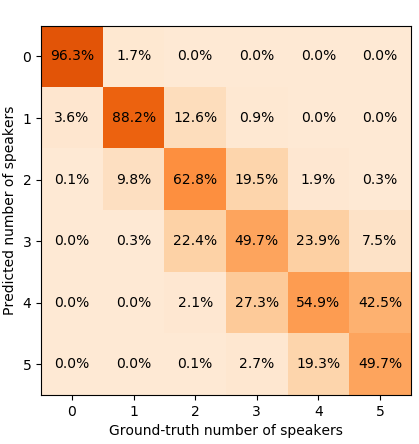
\includegraphics[width=.4\textwidth]{Images/chap5/conf_mat_3_3_10frames_simulatedSRIRs.png} \label{subfig:cm_3_3_10frames}}
    \subfloat[Kernels $3 \times 3$,\\ 20 frames]{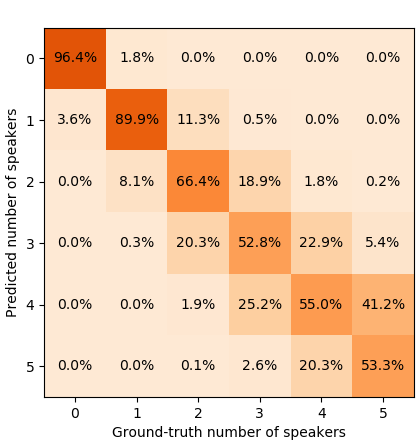
\includegraphics[width=.4\textwidth]{Images/chap5/conf_mat_3_3_20frames_simulatedSRIRs.png} \label{subfig:cm_3_3_20frames}}
    \subfloat[Kernels $3 \times 3$,\\ 30 frames]{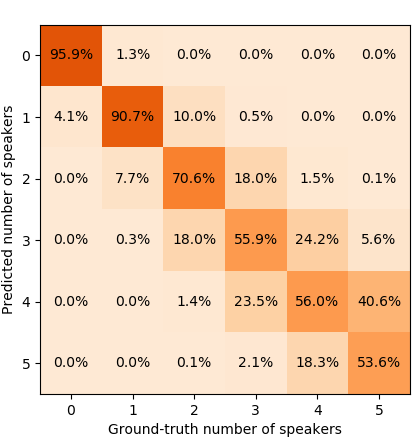
\includegraphics[width=.4\textwidth]{Images/chap5/conf_mat_3_3_30frames_simulatedSRIRs.png} \label{subfig:cm_3_3_30frames}}}\\
    
    \makebox[\textwidth][c]{
    \subfloat[Kernels $5 \times 5$,\\ 10 frames]{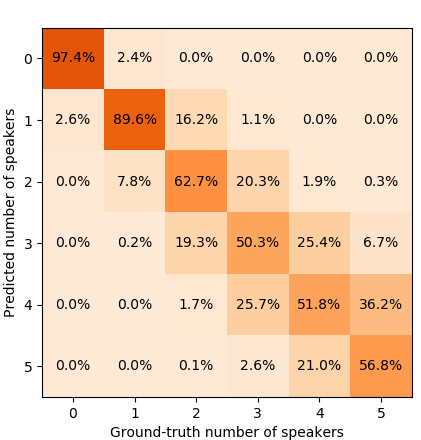
\includegraphics[width=.4\textwidth]{Images/chap5/conf_mat_5_5_10frames_simulatedSRIRs.png} \label{subfig:cm_5_5_10frames}}
    \subfloat[Kernels $5 \times 5$,\\ 20 frames]{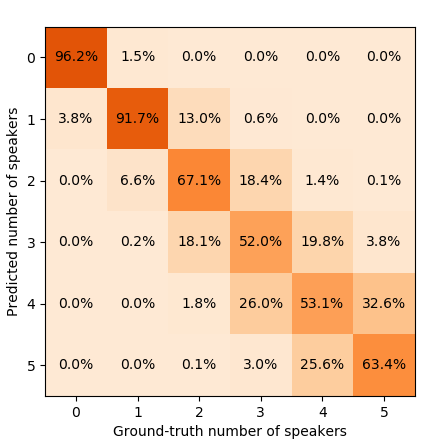
\includegraphics[width=.4\textwidth]{Images/chap5/conf_mat_5_5_20frames_simulatedSRIRs.png} \label{subfig:cm_5_5_20frames}}
    \subfloat[Kernels $5 \times 5$,\\ 30 frames]{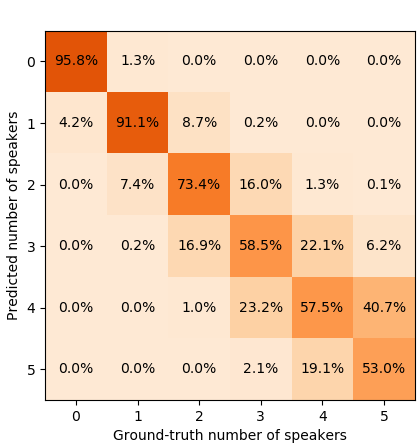
\includegraphics[width=.4\textwidth]{Images/chap5/conf_mat_5_5_30frames_simulatedSRIRs.png} \label{subfig:cm_5_5_30frames}}}\\
    
    \makebox[\textwidth][c]{
    \subfloat[Kernels $7 \times 7$,\\ 10 frames]{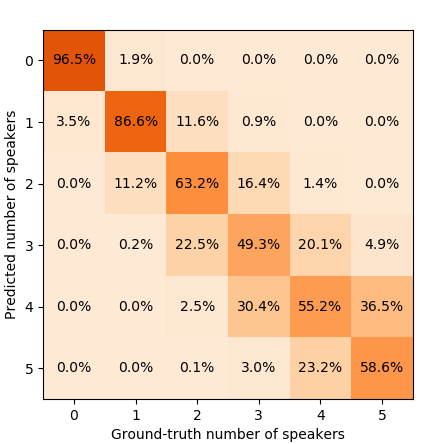
\includegraphics[width=.4\textwidth]{Images/chap5/conf_mat_7_7_10frames_simulatedSRIRs.png} \label{subfig:cm_7_7_10frames}}
    \subfloat[Kernels $7 \times 7$,\\ 20 frames]{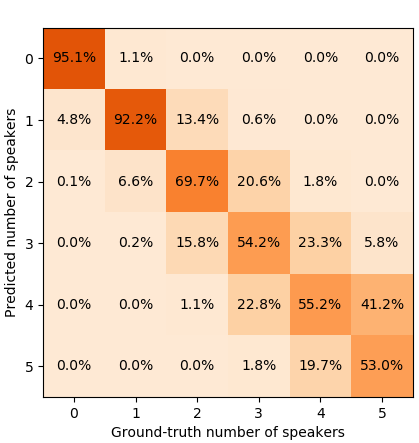
\includegraphics[width=.4\textwidth]{Images/chap5/conf_mat_7_7_20frames_simulatedSRIRs.png} \label{subfig:cm_7_7_20frames}}
    \subfloat[Kernels $7 \times 7$,\\ 30 frames]{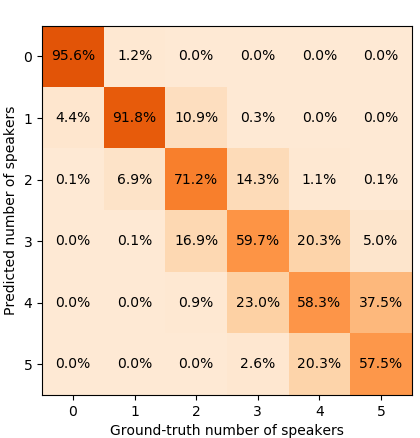
\includegraphics[width=.4\textwidth]{Images/chap5/conf_mat_7_7_30frames_simulatedSRIRs.png} \label{subfig:cm_7_7_30frames}}}
    
    \captionof{figure}[Confusion matrix $A_{ij}$ of the multi-channel speaker counting CRNN on the test dataset, for several values of $(K \times K)$]{Confusion matrices of the accuracy $A_{ij}$ of the proposed speaker counting multi-channel CRNN, evaluated on the test dataset, for convolution kernels of size $3 \times 3$ (top), $5 \times 5$ (middle row), and $7 \times 7$ (bottom), and for an input sequence length $T=10$ frames (left), $20$ frames (middle column), and $30$ frames (right).}
    \label{fig:confusionMatricesKernelSizes}
\end{figure}

\pagebreak

\begin{figure}[t]
    \centering
    \makebox[\textwidth][c]{
    \subfloat[Kernels $3 \times 3$,\\ 10 frames]{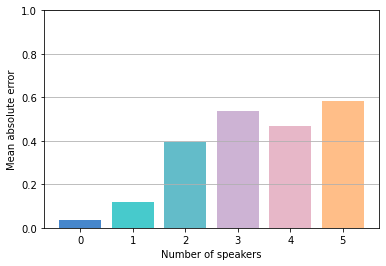
\includegraphics[width=.4\textwidth]{Images/chap5/mae_3_3_10frames_simulatedSRIRs.png} \label{subfig:mae_3_3_10frames}}
    \subfloat[Kernels $3 \times 3$,\\ 20 frames]{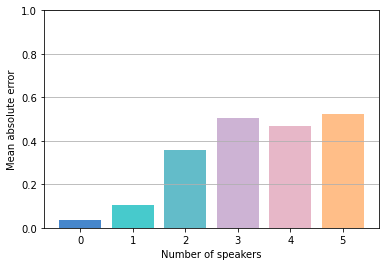
\includegraphics[width=.4\textwidth]{Images/chap5/mae_3_3_20frames_simulatedSRIRs.png} \label{subfig:mae_3_3_20frames}}
    \subfloat[Kernels $3 \times 3$,\\ 30 frames]{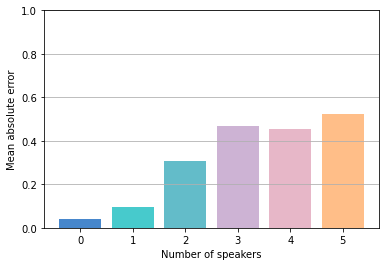
\includegraphics[width=.4\textwidth]{Images/chap5/mae_3_3_30frames_simulatedSRIRs.png} \label{subfig:mae_3_3_30frames}}}\\
    
    \makebox[\textwidth][c]{
    \subfloat[Kernels $5 \times 5$,\\ 10 frames]{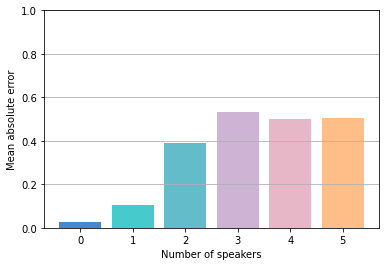
\includegraphics[width=.4\textwidth]{Images/chap5/mae_5_5_10frames_simulatedSRIRs.png} \label{subfig:mae_5_5_10frames}}
    \subfloat[Kernels $5 \times 5$,\\ 20 frames]{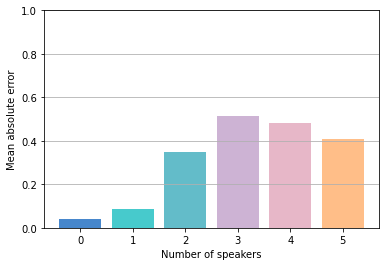
\includegraphics[width=.4\textwidth]{Images/chap5/mae_5_5_20frames_simulatedSRIRs.png} \label{subfig:mae_5_5_20frames}}
    \subfloat[Kernels $5 \times 5$,\\ 30 frames]{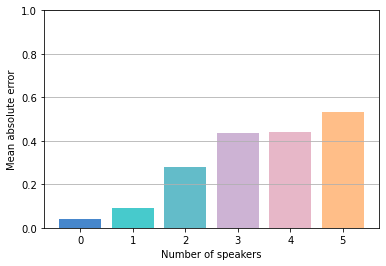
\includegraphics[width=.4\textwidth]{Images/chap5/mae_5_5_30frames_simulatedSRIRs.png} \label{subfig:mae_5_5_30frames}}}\\
    
    \makebox[\textwidth][c]{
    \subfloat[Kernels $7 \times 7$,\\ 10 frames]{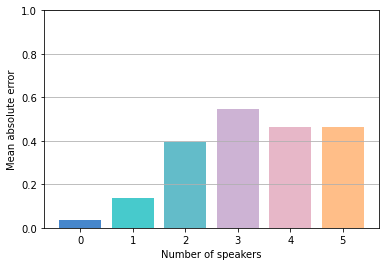
\includegraphics[width=.4\textwidth]{Images/chap5/mae_7_7_10frames_simulatedSRIRs.png} \label{subfig:mae_7_7_10frames}}
    \subfloat[Kernels $7 \times 7$,\\ 20 frames]{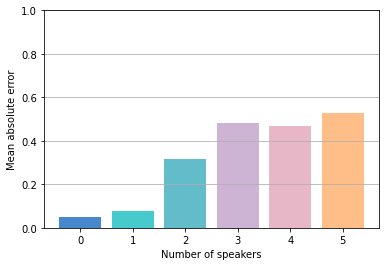
\includegraphics[width=.4\textwidth]{Images/chap5/mae_7_7_20frames_simulatedSRIRs.png} \label{subfig:mae_7_7_20frames}}
    \subfloat[Kernels $7 \times 7$,\\ 30 frames]{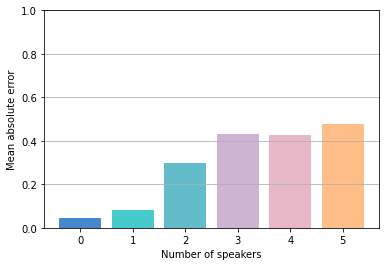
\includegraphics[width=.4\textwidth]{Images/chap5/mae_7_7_30frames_simulatedSRIRs.png} \label{subfig:mae_7_7_30frames}}}
    
    \captionof{figure}[Mean absolute errors $M_i$ of the multi-channel speaker counting CRNN on the test dataset, for several values of $(K \times K)$]{Mean absolute errors $M_i$ of the multi-channel speaker counting CRNN on the test dataset, for several values of $(K \times K)$.}
    \label{fig:maeKernelSizes}
\end{figure}

\clearpage
\subsection{Counting accuracy profile along the sequence}
\label{ss:accuracyAlongTheSequence}

\subsubsection{Experiment objective}

After analyzing the effect of the sequence length $T$ and noticing that the network performance is better when $T$ increases, we concluded that the LSTM layer makes better predictions if it can rely on more past frames. Moreover, we recall the reader that we use the LSTM in a sequence-to-sequence manner (\emph{i.e.}, the LSTM makes a prediction at each timestep, using the processing of the previous timesteps). Therefore, one can legitimately think that making a prediction in the beginning of the input sequence will generally be less accurate than a prediction at the end of the sequence.

To verify this idea, we measure the overall categorical accuracy $A$ regardless of the class, for an estimate at each frame position in the sequence. This frame-wise accuracy is defined by:
\begin{equation}
    \label{eq:overallCountingCategoricalAccuracy}
    A(\tau) = \frac{\sum_{i=0}^6 \lvert T_i \rvert A_{ii}(\tau)}{\sum_{i=0}^6 \lvert T_i \rvert},
\end{equation}
where $A_{ii}(\tau)$ is the accuracy calculated only from the estimates for frames $\tau$ in a sequence. That is, for all test sequences, we only keep the prediction for the frame position $\tau$ to compute the accuracy $A(\tau)$. We do that for all $\tau \in [1, T]$ and end up with the accuracy $A(\tau)$ as a function of the frame position $\tau$. To perform a fair evaluation on all frames of all test sequences, instead of extracting non-overlapping sequences of $T$ frames from the $15$~s test signals as we did in our previous experiment, here we actually extract the input features with an overlap of $T-1$ (\emph{i.e.}, we shift the input sequence by one frame at a time).

The evaluation of $A(\tau)$ is done for several values of $T \in \{10, 20, 30, 50\}$. We also vary the convolution kernel size, with values $3 \times 3$, $5 \times 5$ and $7 \times 7$, which has been shown to be very interesting for the analysis.

\subsubsection{Results}

\begin{figure}[t]
    \centering
    \makebox[\textwidth][c]{
    \subfloat[$K=3$]{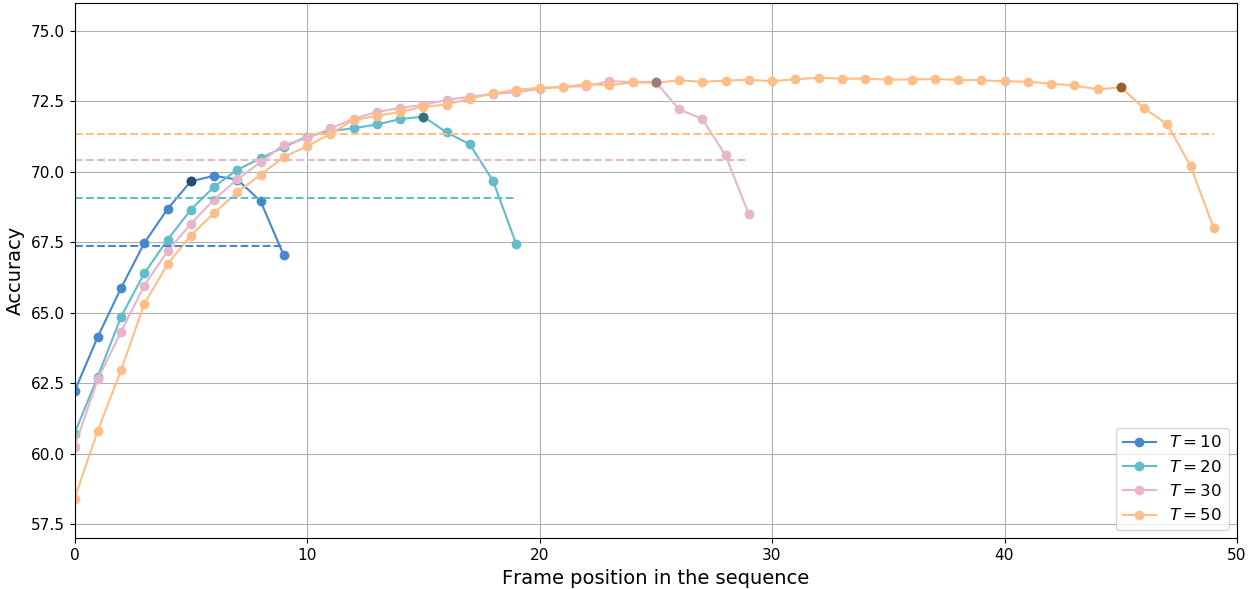
\includegraphics[height=0.28\textheight]{Images/chap5/accuracy_per_frame_3_3_v2.png} \label{subfig:accuracyPerFrame_3_3}}}\\
    
    \makebox[\textwidth][c]{
    \subfloat[$K=5$]{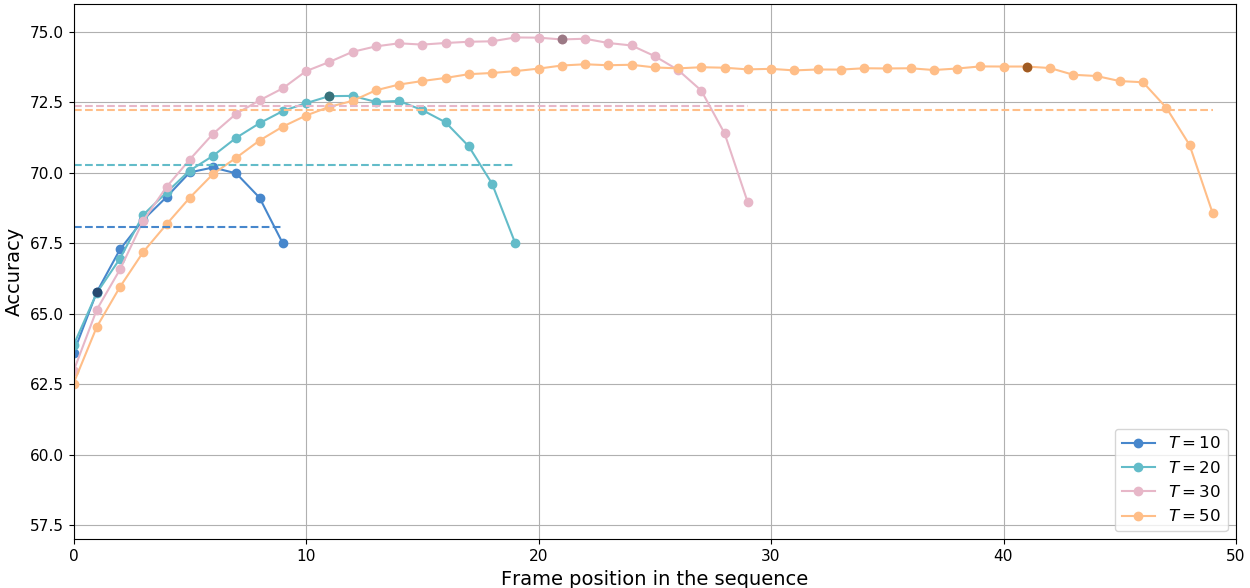
\includegraphics[height=0.28\textheight]{Images/chap5/accuracy_per_frame_5_5_v2.png} \label{subfig:accuracyPerFrame_5_5}}}\\
    
    \makebox[\textwidth][c]{
    \subfloat[$K=7$]{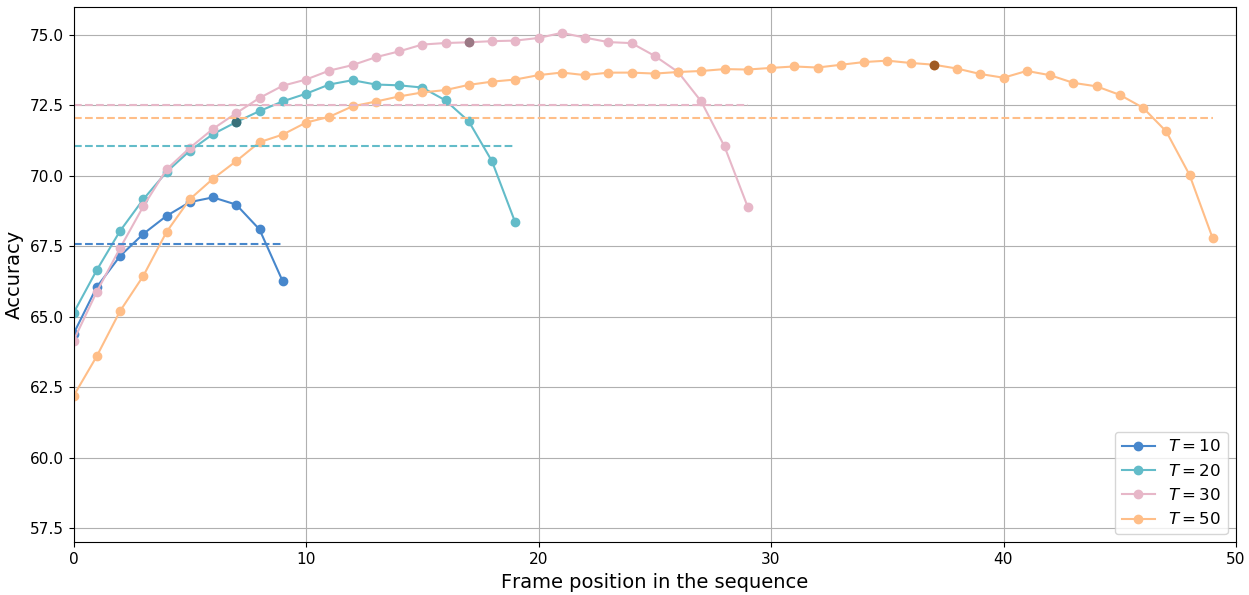
\includegraphics[height=0.28\textheight]{Images/chap5/accuracy_per_frame_7_7_v2.png} \label{subfig:accuracyPerFrame_7_7}}}\\

    \captionof{figure}[Overall accuracy according to the predicted frame position in the input sequence, for $K=3,5,7$]{Overall accuracy according to the predicted frame position in the input sequence, for $K=3$ (top), $K=5$ (middle) and $K=7$ (bottom). On each plot we show the frame-wise accuracy for different sequence length $T$, with a darker value representing the empirical optimal frame position. In horizontal dashed lines are represented the average accuracy on all frame positions.}
    \label{fig:accuracyPerFrame}
\end{figure}

Fig.~\ref{fig:accuracyPerFrame} displays the accuracy $A(\tau)$ as a function of the frame position $\tau$ in the input sequence of size $T$, for several values of $T \in \{10,20,30,50\}$ (represented with different colors) as well as three convolution kernel sizes $K \in \{3,5,7\}$ (corresponding to the three subplots). The overall accuracy, averaged over all frame positions, is also represented with the horizontal dashed lines for the reference.

The first observation we can make is that all curves present a similar shape, with first a rise of the accuracy $A(\tau)$ when $\tau$ increases from $0$, then $A(\tau)$ reaches a maximum, and possibly a plateau in the middle values of $\tau$, and finally $A(\tau)$ decreases when $\tau$ gets close to $T$. Part of this shape can be explained as an expected behavior from the LSTM layer. The increase in accuracy for the first values of $\tau$ can be interpreted as the fact that the LSTM needs a certain amount of past information to make a correct prediction. This rise is indeed quite important for the first values of $\tau$. When $K=3$ and $T=10$, the accuracy goes from $62.5$\% for $\tau=0$ to $70$\% for $\tau=6$. For $K=5$ and $T=50$, $A(\tau)$ goes from $62.5$\% for $\tau=0$ to around $74$\% at $\tau=20$, and then we observe a plateau for the accuracy. This plateau is noticeable (and possibly large) only for high values of $T$, and seems to indicate the convergence of the LSTM. For small $T$, one can think that the LSTM does not reach this convergence when the accuracy starts decreasing, due to another phenomenon, detailed below. To sum up, we can conclude that the LSTM needs a certain amount of past information for a good prediction, leading to a notable increase in prediction accuracy.

Whether the accuracy reaches a plateau (for large enough values of $T$) or a local maximum (for small $T$), we always see an important decrease when $\tau$ gets close to $T$. This means that the network predictions for the last frames of the input sequence are less accurate that for the middle frames, however better than for the very first frames. For instance, for $K=3$, we notice that the accuracy starts decreasing for $\tau=T-5$ for all $T$, except for $T=10$ where the accuracy starts decreasing at $\tau=T-3$. For $K=5$, the accuracy decrease happens for $\tau=T-9$ except for $T=10$. For $K=7$ the drop is less similar depending on $T$: we observe it for $\tau=T-10$ when $T=30$ and for $\tau=T-16$ when $T=50$. So it seems that the position where the accuracy starts decreasing is correlated to the size of the convolution kernels. In fact, we conjecture that it is due to the use of zero-padding in the convolutional layers. This technique, used to preserve the shape of the input feature, adds frames of zeroes before and after the input sequence (and zero-valued frequency bins also) so that the kernels can be applied at the edge of the spectrogram. It results in a convolution operation done on the edge regions where part of the processed data does not contain any information (\emph{i.e.}, filled with zeroes), so the resulting vectors would contain less information for the next layer. As this effect happens for all convolutional layers, the number of zero-valued frames added at the beginning and end of the input features is related to the number of convolutional layers and the corresponding kernel sizes $K$. In our case, as there are $4$ convolutional layers in our CRNN, $4 \times \frac{K-1}{2} = 2K-2$ zero-valued frames are added before and after the input feature. Thus we can expect a decrease in accuracy, due the LSTM process on vectors with less information, starting from the frame at position $2K-2$ before the end of the sequence.

Finally, due to the LSTM behavior and the use of zero-padding in all $4$ convolutional layers, an empirical formula can be draw to express the optimal position $\tau_{opt}$ for a frame in the sequence, to obtain the best prediction (a sequence starts at $\tau=0$):
\begin{equation}
    \tau_{opt} = T-2K+1.
\end{equation}

This empirical optimal position is showed in darker color in Fig.~\ref{fig:accuracyPerFrame}.

To conclude, this simple performance analysis shows that the use of LSTM layers and zero-padding in convolutional layers results in an asymmetrical prediction accuracy depending on the position of the analyzed frame in the input sequence. We notice that a gain of $10$\% in accuracy can be obtained by choosing the optimal frame position, which we try to justify by inspecting the behavior of neural network components. To illustrate the prediction power of our speaker counting system, we show in Fig.~\ref{fig:predictionExample} the predicted and ground-truth NoS of three $15$-s mixtures, with $1$, $3$ and $5$ speakers, respectively. We use the neural network with $K = 5$, and a sequence length $T=30$. Using an overlap of $T-1$, we successively extract the input features from the $15$-s mixtures and keep only the prediction for the frame $\tau = \tau_{opt}$.\footnote{As we do not use zero-padding, for the input feature extracted at the very beginning of the mixture we keep all predictions for $\tau < \tau_{opt}$, and for the input feature extracted at the very end we keep all predictions for $\tau > \tau_{opt}$.} We therefore estimate the NoS for all frames in the mixtures. In the top plot of Fig.~\ref{fig:predictionExample}, ($1$-speaker signal), the prediction is almost perfect, but we notice that the network failed to capture a short speech break around frame $300$, and seems to be sometimes a bit early or late by a few frames in its prediction (\emph{e.g.}, around frames $75$ and $360$). In the middle plot ($3$-speaker signal), the predictions are less accurate than with $1$ speaker but still relatively precise. We also notice a few predictions time-shifted from the ground-truth (\emph{e.g.}, around frame $80$ and sometimes the network does not detect a new speaker (\emph{e.g.}, around frame 160). Moreover, in different frame regions (\emph{e.g.}, around frames $210$ and $330$), the network overestimates the number of speakers. In the bottom plot ($5$-speaker signal), the prediction performance is degraded, as expected due to the increasing complexity of the task. Still, we see that the predictions lie around the ground-truth.

\begin{figure}[t]
    \begin{center}
    \makebox[\textwidth][c]{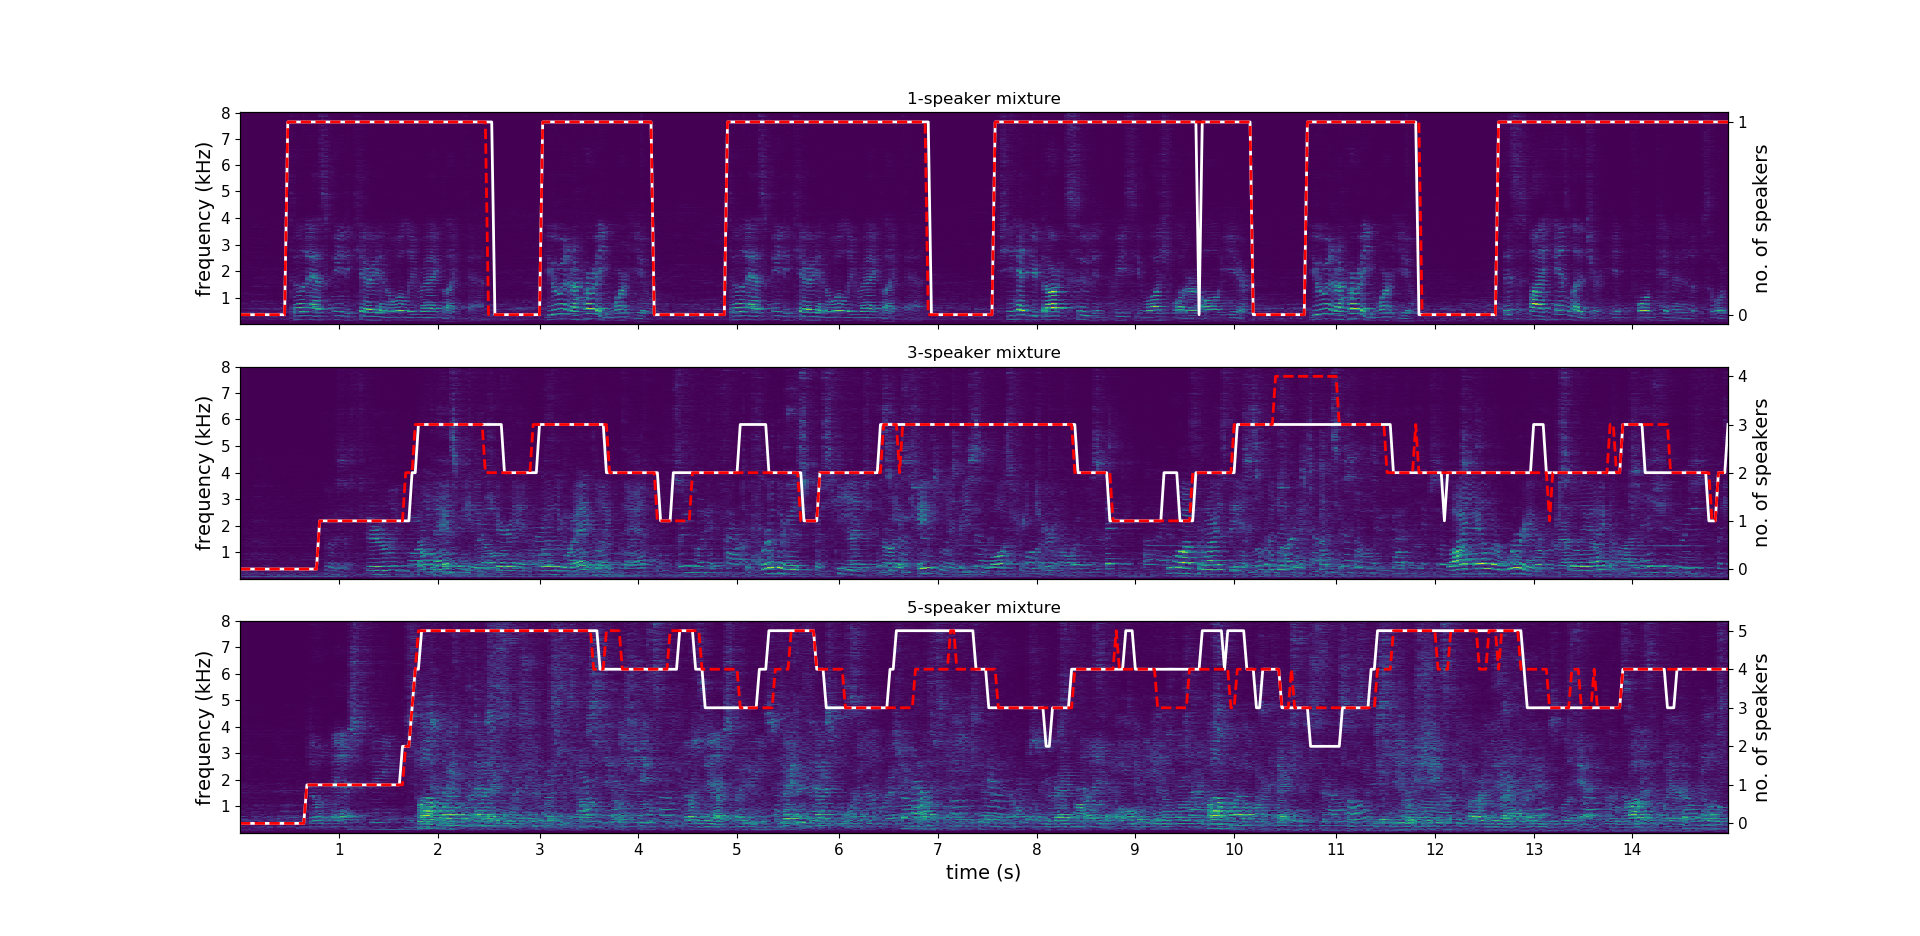
\includegraphics[width=1.5\linewidth]{Images/chap5/predictionExample.png}}
    \captionof{figure}[Spectrograms with the predicted and ground-truth NoS for three $15$-s test mixtures]{Spectrograms of the $W$ channels of three test signals (with $1$, $3$ and $5$ speakers), with the ground-truth NoS (in white) and the NoS predicted by the proposed multi-channel CRNN (in red). The prediction is based on the result provided by the network at frame $\tau_{opt}$ (see text).}
    \label{fig:predictionExample}
    \end{center}
\end{figure}

%-----------------------------------------------
%  CONCLUSION AND PERSPECTIVES
%-----------------------------------------------
\clearpage
\section{Conclusion and perspectives}

In this chapter, we have introduced a CRNN which is capable of counting up to $5$ speakers in a FOA signals, with a frame-wise resolution. This latter point is a notable difference with the existing state-of-the-art at the time of the presented study. The best speaker counting system available at that time \cite{stoter_countnet:_2019} was providing the maximum NoS over 5s-mixtures.

Our CRNN, trained on FOA magnitude spectrogram is composed of several convolutional layers, which are designed to extract spectral and spatial information while preserving the temporal dimension, followed by a sequence-to-sequence LSTM layer and an output feedforward layer. The $6$ softmax neurons of the output layer estimate a probability distribution over the NoS (from $0$ to $5$) for each frame in the input spectrogram. The evaluation of this speaker counting CRNN on simulated data showed that it can classify a multi-channel signal as being non-speech with almost perfect accuracy, and is able to estimate the presence of $1$ speaker around $90$\% precision. When the number of speakers is greater or equal to $2$, the accuracy is still greater than $50\%.$

We conducted several experiments in order to assess the benefit of certain hyperparameters. First, we showed the superiority of using multi-channel features over single-channel ones, suggesting the benefit of spatial information for speaker counting. We noticed that the network accuracy increased when the length of the input sequence was larger, and it seemed that augmenting the convolution kernel sizes slightly helped for better predictions but this was not fully conclusive. Finally, we carried out a performance analysis which showed that the network prediction accuracy was uneven for all frames in a given sequence, due to the LSTM behavior and the use of zero-padding in the convolutional layers. Based on an empirical investigation, we concluded that the best counting accuracy is obtained for the last frames in the sequence which are not affected by zero-padding.

Although some design efforts have been made to improve the counting accuracy, as well as an analysis to assess the network performance, there is still room for future investigation in many aspects. While only a small number of convolutional layers has been used here, we believe that the feature extraction stage could be easily improved, based on one experiment we conducted for DoA estimation \ref{ss:multiLocalizationfeatureExtractionModule}. Regarding this, several aspect could be investigated, such as the number of convolutional layers, the convolutional shapes (2D, 3D), the use of dilated kernels, or even the addition of residual connections which might help if numerous layers are used. A better feature extraction could lead to a better discrimination between sources, thus leading to a more accurate speaking counting. One may also think of bidirectional layers for an improved temporal analysis. Regarding speaker discrimination, the use of phase information, as well as considering HOA features could further improve the network performance, which was already shown to benefit from spatial information. We think that increasing the Ambisonics order and improving feature extraction are the most promising options for improving the speaker counting performance. Another perspective is to explore a more suitable loss function such as the earth-mover distance \cite{hou_squared_2016}, as it could make a better benefit of the inter-class relationships.
